\documentclass[UTF8,zihao=-4]{ctexrep}

\usepackage[a4paper,left=2.8cm,right=2.5cm,top=2.5cm,bottom=2.5cm]{geometry}
\usepackage{setspace}
\usepackage{graphicx}
\usepackage{float}
\usepackage{hyperref}

\setstretch{1.5}

\begin{document}

\begin{center}
    {\heiti\zihao{2} 基于 Web 的文件上传、下载与删除管理系统设计与实现}
\end{center}

\newpage

\tableofcontents
\newpage

\chapter{绪论}

\section{项目完成情况}

本次课程设计完成了一个基于 Web 的文件管理系统，系统主要围绕文件上传、文件下载和文件删除三个核心功能展开。项目采用 Flask 框架作为后端服务，使用 HTML 和 CSS 设计前端用户界面，并结合 JavaScript 与 jQuery UI 实现页面交互效果。系统整体界面分为两个主要部分：第一部分为文件上传区域，第二部分为文件管理区域，用户可以在文件管理区域查看已上传文件，并对文件进行下载或删除操作。

在功能实现方面，系统已经完成了单文件上传和文件夹上传功能。用户可以通过页面中的文件选择区域选择本地文件，并将文件上传到服务器指定目录中。后端通过 Flask 接收上传请求，并将文件保存到 uploads 文件夹中。除了单文件上传外，系统还实现了文件夹上传功能，用户可以选择整个文件夹进行上传，系统会保留文件夹内部的目录结构，从而提高文件管理的完整性和实用性。

在文件管理方面，系统实现了文件列表显示、文件下载和文件删除功能。后端能够读取服务器端 uploads 目录下的文件和文件夹信息，并将其整理为目录结构数据返回给前端。前端页面根据返回的数据生成文件列表，显示文件名称、文件大小、修改时间等信息。用户点击下载按钮时，可以下载对应文件；如果下载的是文件夹，系统会自动将文件夹压缩为 zip 文件后再提供下载。用户点击删除按钮时，系统会弹出确认对话框，确认后可删除对应的文件或文件夹。

在交互设计方面，系统使用了 jQuery UI 组件库对页面功能进行增强。上传区域使用 Tabs 组件区分单文件上传和文件夹上传；操作按钮使用 Button 组件进行美化；上传过程中使用 Progressbar 组件显示上传状态；ファイル删除前使用 Dialog 组件弹出确认提示，避免用户误删ファイル。通过这些组件的使用，系统界面更加清晰，用户操作也更加直观。

此外，系统还实现了用户注册、登录和退出功能。用户访问系统主页时，如果未登录会跳转到注册或登录页面，登录成功后才能进入文件管理页面。系统使用 JSON 文件保存用户信息，并通过 session 记录用户登录状态。虽然用户管理不是本课程设计题目要求的核心功能，但它可以提高系统的完整性，使文件管理系统更加接近实际 Web 应用。

在安全性和异常处理方面，系统对上传和访问路径进行了规范化处理，避免用户通过特殊路径访问 uploads 目录以外的文件。当用户上传空文件、删除不存在的文件或访问非法路径时，系统能够返回相应的错误提示。整体来看，本项目已经基本完成课程设计要求，实现了基于 HTML、CSS 和 jQuery UI 的文件管理页面，并完成了文件上传、文件下载和文件删除三个主要功能。

\section{课题背景与意义}

随着计算机网络技术和 Web 应用技术的不断发展，越来越多的日常工作开始从本地单机操作转向基于浏览器的在线操作。在学习、办公和软件开发过程中，文件的上传、下载、保存和删除是非常常见的需求。例如，学生在提交课程作业时需要上传实验报告或源代码文件；教师在发布教学资料时需要提供文件下载；在团队协作中，成员之间也经常需要通过网络系统共享文档、图片、压缩包等各种类型的文件。因此，设计并实现一个具有基本文件管理功能的 Web 系统，具有较强的实用价值和学习意义。

传统的文件管理通常依赖操作系统自带的文件资源管理器，用户只能在本地计算机上完成文件查看、复制、删除等操作。这种方式虽然简单直接，但不适合网络环境下的文件共享和远程管理。当用户需要在不同设备之间传输文件，或者希望通过浏览器统一管理服务器上的文件时，就需要借助 Web 文件管理系统。Web 文件管理系统能够通过浏览器提供统一的操作界面，用户不需要直接接触服务器文件目录，也不需要掌握复杂的命令行操作，只需要通过页面按钮即可完成文件上传、文件下载和文件删除等操作。

本课题所设计的文件管理系统正是围绕这一实际需求展开的。系统通过 HTML 和 CSS 完成用户界面设计，将页面划分为文件上传区域和文件管理区域两个主要部分。其中，文件上传区域用于选择并上传本地文件，文件管理区域用于展示服务器端已经保存的文件，并提供下载和删除操作。当前项目中的主页面已经按照这一思路进行设计，页面中包含“上传文件”和“文件列表”两个核心区域，其中上传区域又分为单个文件和整个文件夹两个选项，文件列表区域则展示文件名称、大小、修改时间以及操作按钮等信息。这种设计能够使用户较为清晰地理解系统功能，也便于后续进行功能扩展。

在前端交互方面，本课题要求使用 jQuery UI。jQuery UI 是基于 jQuery 的用户界面组件库，提供了按钮、对话框、选项卡、进度条等常用界面组件。相比于只使用普通 HTML 表单和浏览器默认提示框，jQuery UI 可以让页面具有更好的交互效果和更统一的视觉风格。在本系统中，上传部分使用选项卡组件区分单文件上传和文件夹上传，按钮组件用于美化上传、刷新、下载和删除等操作按钮，进度条组件用于显示上传过程状态，对话框组件用于显示提示信息和删除确认信息。这些组件的使用使系统不再只是简单的静态页面，而是具有一定交互能力的 Web 应用界面。

从课程设计的角度来看，本课题能够综合运用前端页面设计、后端接口开发、文件系统操作和前后端交互等多方面知识。前端部分需要使用 HTML 组织页面结构，使用 CSS 控制页面布局和样式，并使用 JavaScript 与 jQuery UI 实现用户交互；后端部分需要使用 Flask 框架接收浏览器请求，完成文件保存、文件读取、文件下载和文件删除等操作；同时还需要考虑文件路径处理、异常提示、页面刷新和用户操作反馈等问题。因此，该课题不是单一知识点的简单练习，而是一个具有完整功能流程的小型 Web 应用项目。

本课题的意义主要体现在以下几个方面。首先，通过实现文件上传、下载和删除功能，可以加深对 Web 请求与响应过程的理解。文件上传需要浏览器将本地文件通过表单或 Ajax 请求提交给服务器，服务器接收后再保存到指定目录；文件下载则需要服务器将指定文件作为响应内容返回给浏览器；文件删除则涉及前端确认、后端定位文件以及执行删除操作等步骤。通过这些功能的实现，可以更加直观地理解浏览器与服务器之间的数据交互过程。

其次，本课题有助于提高前端界面设计能力。一个可用的系统不仅要能完成后台功能，还需要有清晰、友好的用户界面。通过本系统的设计，可以学习如何将页面划分为不同功能区域，如何设计上传框、文件列表、操作按钮和提示对话框，如何使用 CSS 控制布局、间距、颜色和响应式效果。同时，jQuery UI 组件的使用也可以帮助理解前端组件化思想，即通过封装好的组件提高开发效率和界面一致性。

再次，本课题能够锻炼后端开发和文件操作能力。文件管理系统虽然规模不大，但涉及的后端逻辑比较完整，包括接收上传文件、创建保存目录、遍历服务器文件夹、返回文件列表数据、判断文件或文件夹类型、压缩文件夹、删除文件或目录等内容。这些操作都与实际 Web 系统中的资源管理功能密切相关。通过本课题的实现，可以进一步理解 Flask 路由、请求对象、响应对象以及服务器端文件系统操作的基本方法。

最后，本课题还具有一定的实际应用价值。虽然本系统属于课程设计项目，功能规模相对较小，但它已经具备了一个基础文件管理平台的主要功能。在此基础上，后续可以继续扩展用户权限管理、文件分类管理、文件预览、文件搜索、上传进度显示、文件大小限制、数据库存储和多用户隔离等功能，使系统更加接近真实场景中的在线文件管理平台。因此，本课题不仅能够满足课程设计对 HTML、CSS、jQuery UI 和文件操作功能的要求，也为后续学习更复杂的 Web 应用开发打下基础。

\section{文件管理系统介绍}

\subsection{系统主要功能}

本系统是一个基于 Web 的文件管理工具，主要围绕文件的日常管理需求进行设计，提供文件上传、文件下载和文件删除三个核心功能。

在文件上传方面，系统支持单文件上传和整个文件夹上传两种方式。单文件上传允许用户选择本地计算机中的任意一个文件并将其上传至服务器的指定存储目录中；文件夹上传则允许用户选择整个文件夹，系统会自动读取文件夹内的所有文件及其相对路径，并将目录结构完整地保存到服务器端。这两种上传方式可以满足不同场景下的文件传输需求。

在文件下载方面，系统支持单个文件下载和文件夹下载两种形式。对于单个文件，用户点击下载按钮后，浏览器会直接从服务器获取文件并保存到本地。对于文件夹，系统会先将文件夹中的所有文件打包成一个 zip 压缩包，再提供给用户下载，从而保证文件夹内的目录结构不会丢失。

在文件删除方面，系统提供文件删除和文件夹删除功能。用户在查看文件列表时，可以对不需要的文件或文件夹执行删除操作。为防止用户误操作，系统在执行删除之前会弹出确认对话框，用户确认后方可完成删除。删除操作会从服务器存储目录中彻底移除对应的文件或文件夹。

除了上述三个核心功能外，系统还实现了用户注册、登录和退出功能。用户首次使用时需要注册一个账号，之后通过登录进入系统主页。退出功能使用户可以安全地结束当前会话。用户管理虽然不是本系统的核心功能要求，但它为系统提供了基本的访问控制能力，使不同用户的使用环境相互隔离。

\subsection{系统操作方式}

用户通过浏览器访问系统主页。如果用户尚未登录，系统会自动跳转到注册或登录页面。新用户需要填写用户名和密码完成注册，注册成功后跳转到登录页面，输入正确的账号和密码后方可进入文件管理主页面。

系统主页面以左右两栏布局呈现。页面左侧为文件上传区域，右侧为文件管理区域，两个区域在功能上相互独立，便于用户同时进行上传和管理操作。

在文件上传区域中，系统使用选项卡组件将上传方式划分为单个文件上传和整个文件夹上传两个标签页。默认显示的是单文件上传标签页，用户可以通过点击选项卡切换到文件夹上传标签页。每个标签页内都有一个文件选择区域，用户点击该区域或拖拽文件到区域中即可选择要上传的内容。在选择文件后，页面上会显示已选择的文件名称或文件夹中的文件数量，确认无误后点击上传按钮即可将文件发送至服务器。上传过程中，进度条会实时显示上传进度。

在文件管理区域中，系统以列表形式展示服务器端存储的所有文件和文件夹。列表中的每一行代表一个文件或文件夹，依次显示名称、大小和修改时间。对于文件夹，用户可以通过点击名称前的箭头图标展开或折叠文件夹，查看其中的子文件和子文件夹。每个文件或文件夹右侧都对应有下载和删除两个操作按钮。用户点击下载按钮即可将文件保存到本地；点击删除按钮会弹出确认对话框，用户确认后才会执行删除操作。文件列表还提供了刷新按钮，用户可以随时刷新列表以获取最新的文件状态。系统的主页面布局如图~\ref{fig:file_control} 所示。

\begin{figure}[H]
    \centering
    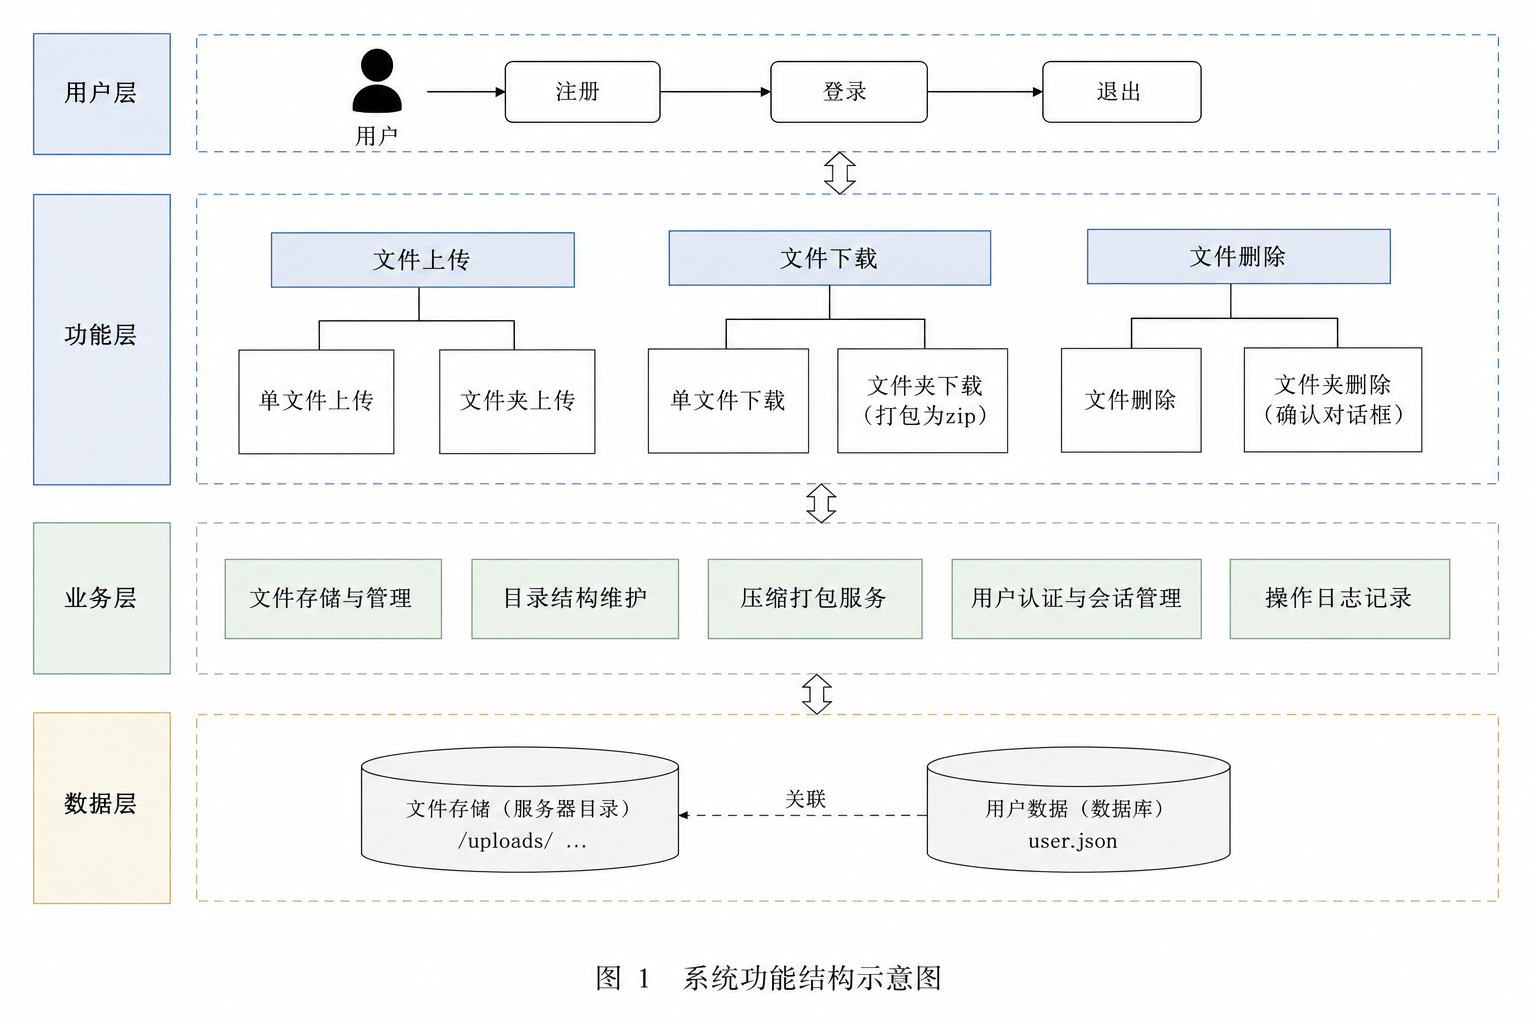
\includegraphics[width=0.95\textwidth]{figures/file_control.png}
    \caption{文件管理系统主页面}\label{fig:file_control}
\end{figure}

\section{相关开发技术介绍}

\subsection{HTML 与 CSS 技术介绍}

\subsection{jQuery UI 技术介绍}

\subsection{Flask 框架介绍}


\chapter{系统分析}

\section{需求分析}

\subsection{文件上传需求}

\subsection{文件下载需求}

\subsection{文件删除需求}

\section{功能分析}

\subsection{基本功能}

\subsection{拓展功能}

\section{系统结构分析}

本系统采用浏览器/服务器（B/S）架构，分为前端浏览器层和后端服务器层两层结构。前端负责用户界面展示与交互操作，后端负责业务逻辑处理与数据存储，两层之间通过 HTTP 协议进行通信。系统的整体结构如图~\ref{fig:architecture} 所示。

\begin{figure}[H]
    \centering
    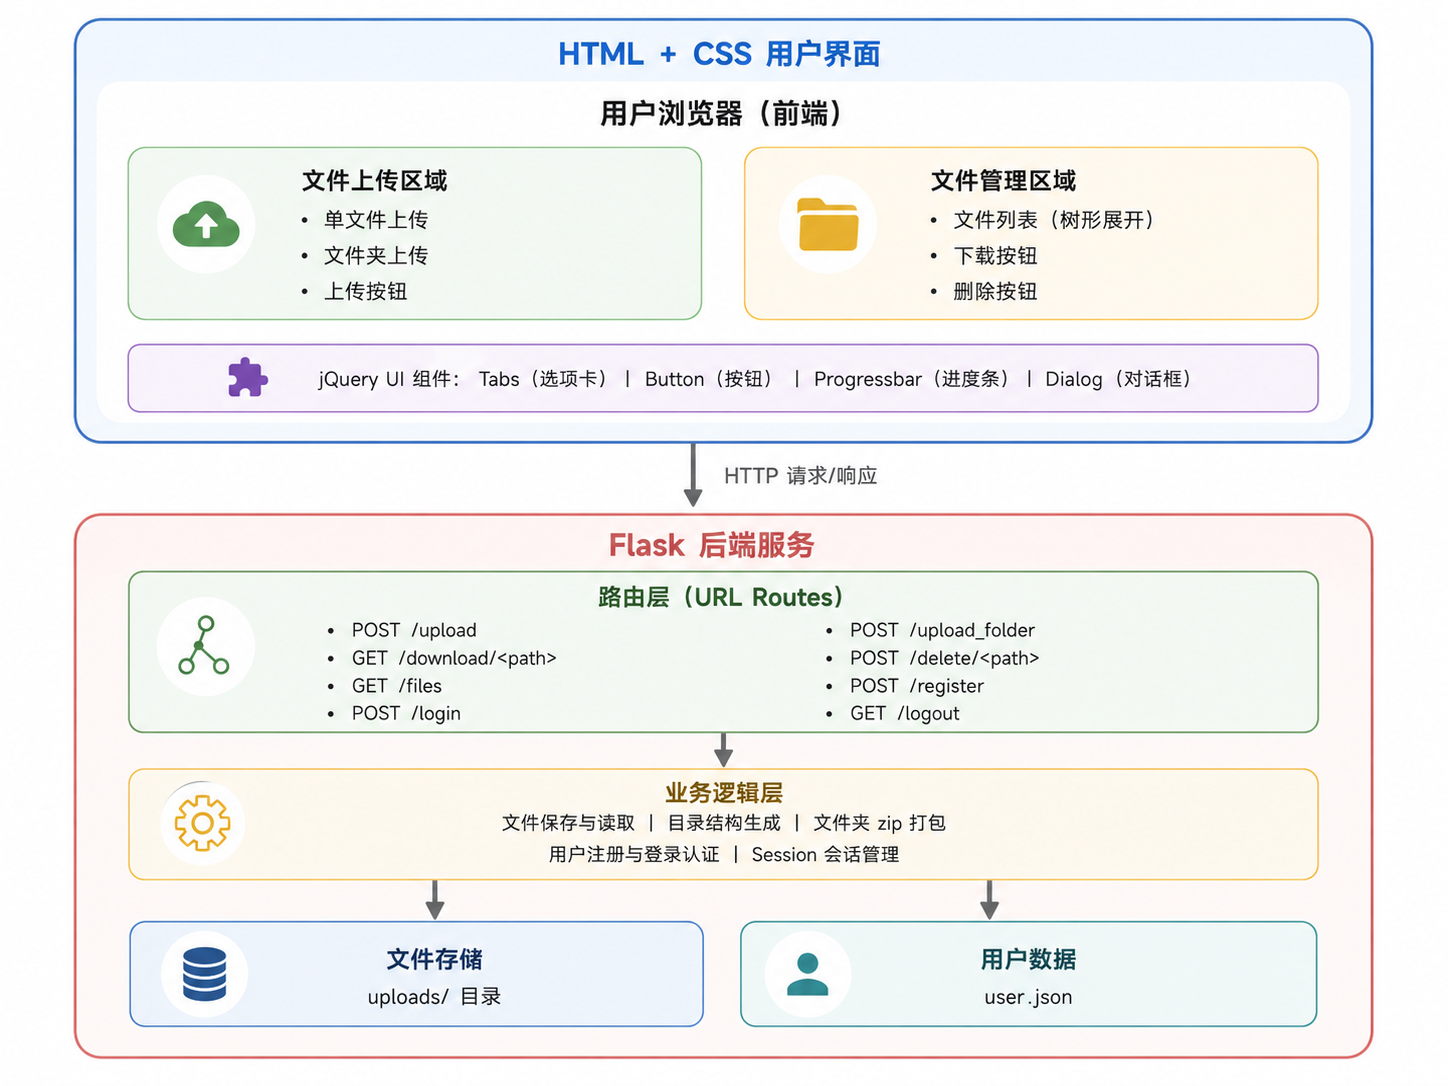
\includegraphics[width=0.92\textwidth]{figures/system_architecture.png}
    \caption{系统整体结构图}\label{fig:architecture}
\end{figure}

前端运行在用户浏览器中，由 HTML 和 CSS 构建用户界面。页面主要划分为两个功能区域：文件上传区域和文件管理区域。文件上传区域提供单文件上传和文件夹上传两种方式，用户可通过选项卡切换。文件管理区域以列表形式展示服务器端的文件与文件夹信息，并提供下载和删除操作按钮。前端交互功能基于 jQuery UI 组件库实现，包括选项卡（Tabs）、按钮（Button）、进度条（Progressbar）和对话框（Dialog）等组件，以增强用户操作体验。

后端基于 Flask 框架实现，负责接收前端请求并执行相应的业务逻辑。路由层定义了系统提供的全部 URL 接口，包括文件上传、文件夹上传、文件下载、文件删除、文件列表获取以及用户注册、登录和退出等路由。业务逻辑层处理文件保存与读取、路径安全校验、文件夹压缩打包、用户认证和会话管理等核心逻辑。数据存储层包含两个部分：文件存储使用服务器文件系统中的 uploads 目录保存所有上传的文件和文件夹；用户数据使用 JSON 文件保存注册用户的账号信息。系统通过分层设计实现了前后端分离，各层职责清晰，便于后续功能的扩展与维护。

\chapter{详细设计及实现}

\section{系统总体设计}

\section{用户界面设计}

\subsection{文件上传区域设计}

\subsection{文件管理区域设计}

\section{jQuery UI 组件设计}

\subsection{选项卡组件}

\subsection{按钮组件}

\subsection{进度条组件}

\subsection{对话框组件}

\section{文件上传功能实现}

\section{文件下载功能实现}

\section{文件删除功能实现}

\section{异常处理与安全设计}


\chapter{系统测试}

\section{测试环境}

\subsection{硬件环境}

\subsection{软件环境}

\section{页面显示测试}

\section{文件上传测试}

\section{文件下载测试}

\section{文件删除测试}

\section{异常情况测试}

\section{测试小结}


\chapter{总结与展望}

\section{课程设计总结}

\section{系统不足}

\section{改进方向}


\begin{thebibliography}{99}

\bibitem{html}
MDN Web Docs. HTML: HyperText Markup Language[EB/OL].

\bibitem{css}
MDN Web Docs. CSS: Cascading Style Sheets[EB/OL].

\bibitem{jqueryui}
jQuery UI. jQuery UI Documentation[EB/OL].

\bibitem{flask}
Flask Documentation. Flask Web Development Documentation[EB/OL].

\end{thebibliography}

\end{document}